\documentclass[tikz, border=20pt]{standalone}
\usepackage{helvet}
\renewcommand{\familydefault}{\sfdefault}

\begin{document}

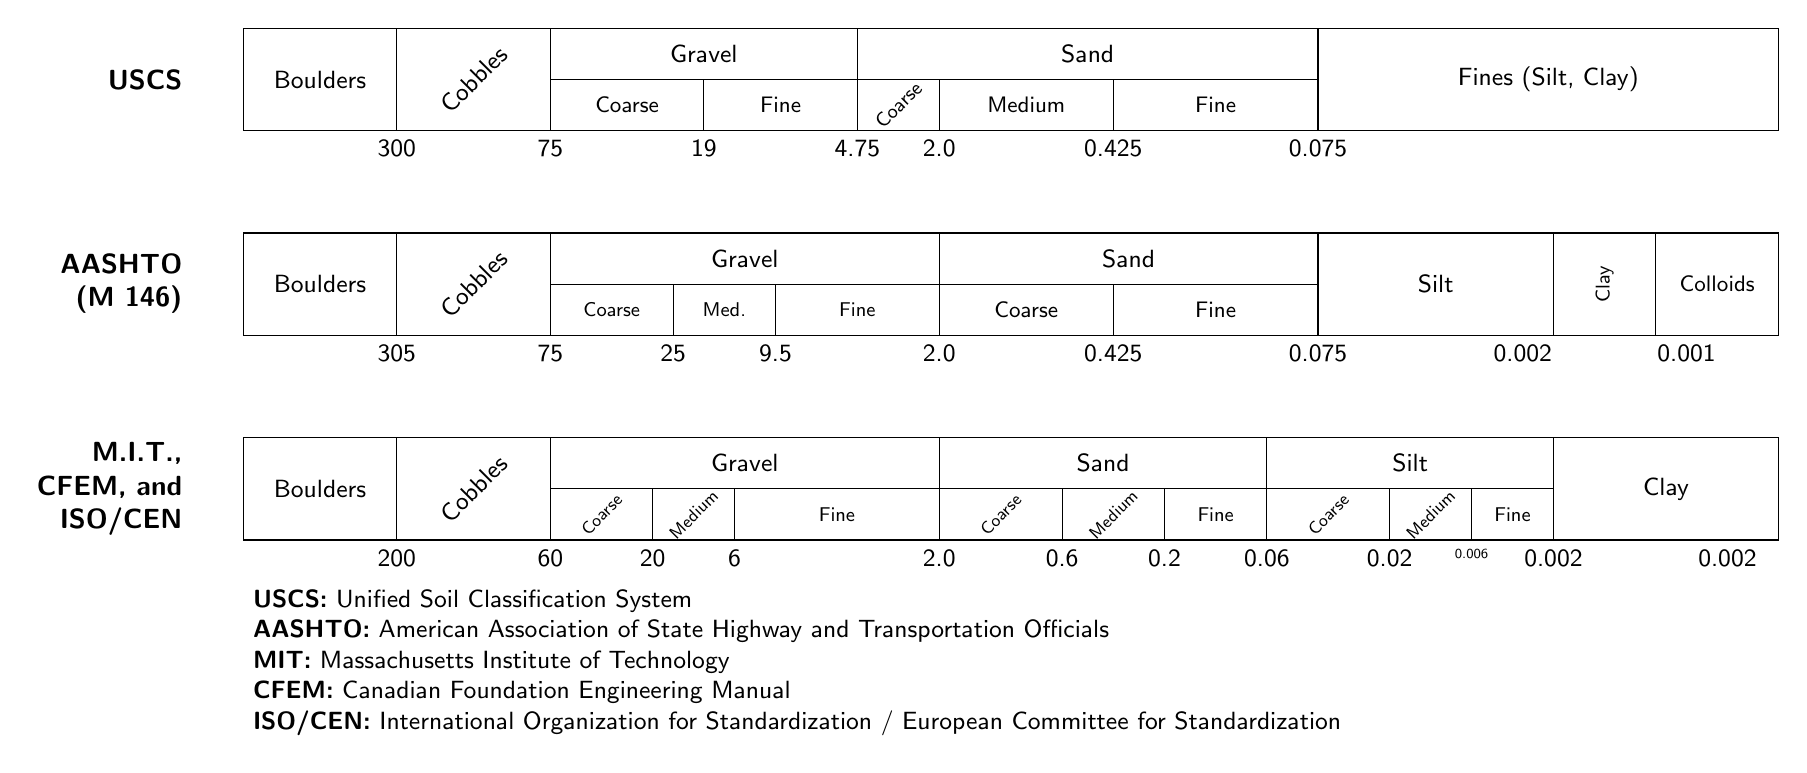
\begin{tikzpicture}[xscale=1.3, yscale=1.3, font=\sffamily\small]

% --- Definitions for vertical positions ---
% We draw from top to bottom
\def\yUSCS{4}
\def\yAASHTO{2}
\def\yMIT{0}
\def\h{1.0} % Height of the bars

% --- X-Coordinates (Manual spacing to fit text) ---
% Left start
\def\xStart{0} 

% Group 1: Boulders/Cobbles boundary
\def\xThreeHundred{1.5}  % 300 / 305
\def\xTwoHundred{1.5}    % 200 is visually aligned here in MIT

% Group 2: Cobbles/Gravel boundary
\def\xSeventyFive{3.0}   % 75
\def\xSixty{3.0}         % 60 (MIT)

% Group 3: Inside Gravel
\def\xTwentyFive{4.2}    % 25 (AASHTO)
\def\xTwenty{4.0}        % 20 (MIT)
\def\xNineteen{4.5}      % 19 (USCS)
\def\xNinePointFive{5.2} % 9.5 (AASHTO)
\def\xSix{4.8}           % 6 (MIT)

% Group 4: Gravel/Sand boundary
\def\xFourSevenFive{6.0} % 4.75 (USCS)
\def\xTwo{6.8}           % 2.0 (Common boundary)

% Group 5: Inside Sand
\def\xZeroSix{8.0}       % 0.6 (MIT)
\def\xZeroFourTwoFive{8.5} % 0.425 (USCS/AASHTO)
\def\xZeroTwo{9.0}       % 0.2 (MIT)

% Group 6: Sand/Fines boundary
\def\xZeroZeroSevenFive{10.5} % 0.075 (USCS/AASHTO)
\def\xZeroZeroSix{10.0}       % 0.06 (MIT)

% Group 7: Inside Silt/Clay
\def\xZeroZeroTwo{11.2}       % 0.02 (MIT)
\def\xZeroZeroZeroSix{12.0}   % 0.006 (MIT)
\def\xZeroZeroZeroTwo{12.8}   % 0.002 (AASHTO boundary is similar)

% Group 8: Clay/Colloids
\def\xZeroZeroZeroOne{13.8}   % 0.001 (AASHTO)
\def\xEnd{15.0}               % End of chart

% ==================================================================
% 1. USCS ROW (Top)
% ==================================================================

% Row Label
\node[anchor=east, font=\bfseries] at (\xStart-0.5, \yUSCS + \h/2) {USCS};

% Boulders
\draw (\xStart, \yUSCS) rectangle (\xThreeHundred, \yUSCS+\h);
\node at (0.75, \yUSCS+\h/2) {Boulders};
\node[below] at (\xThreeHundred, \yUSCS) {300};

% Cobbles
\draw (\xThreeHundred, \yUSCS) rectangle (\xSeventyFive, \yUSCS+\h);
\node[rotate=45] at (2.25, \yUSCS+\h/2) {Cobbles};
\node[below] at (\xSeventyFive, \yUSCS) {75};

% Gravel
\draw (\xSeventyFive, \yUSCS) rectangle (\xFourSevenFive, \yUSCS+\h); % Main box
\draw (\xSeventyFive, \yUSCS+\h/2) -- (\xFourSevenFive, \yUSCS+\h/2); % Mid line
\draw (\xNineteen, \yUSCS) -- (\xNineteen, \yUSCS+\h/2); % Vertical split
\node at ({(\xSeventyFive+\xFourSevenFive)/2}, \yUSCS+0.75) {Gravel};
\node[scale=0.9] at ({(\xSeventyFive+\xNineteen)/2}, \yUSCS+0.25) {Coarse};
\node[scale=0.9] at ({(\xNineteen+\xFourSevenFive)/2}, \yUSCS+0.25) {Fine};
\node[below] at (\xNineteen, \yUSCS) {19};
\node[below] at (\xFourSevenFive, \yUSCS) {4.75};

% Sand
\draw (\xFourSevenFive, \yUSCS) rectangle (\xZeroZeroSevenFive, \yUSCS+\h); % Main box
\draw (\xFourSevenFive, \yUSCS+\h/2) -- (\xZeroZeroSevenFive, \yUSCS+\h/2); % Mid line
\draw (\xTwo, \yUSCS) -- (\xTwo, \yUSCS+\h/2);
\draw (\xZeroFourTwoFive, \yUSCS) -- (\xZeroFourTwoFive, \yUSCS+\h/2);
\node at ({(\xFourSevenFive+\xZeroZeroSevenFive)/2}, \yUSCS+0.75) {Sand};
\node[scale=0.8, rotate=45] at ({(\xFourSevenFive+\xTwo)/2}, \yUSCS+0.25) {Coarse};
\node[scale=0.9] at ({(\xTwo+\xZeroFourTwoFive)/2}, \yUSCS+0.25) {Medium};
\node[scale=0.9] at ({(\xZeroFourTwoFive+\xZeroZeroSevenFive)/2}, \yUSCS+0.25) {Fine};
\node[below] at (\xTwo, \yUSCS) {2.0};
\node[below] at (\xZeroFourTwoFive, \yUSCS) {0.425};
\node[below] at (\xZeroZeroSevenFive, \yUSCS) {0.075};

% Fines
\draw (\xZeroZeroSevenFive, \yUSCS) rectangle (\xEnd, \yUSCS+\h);
\node at ({(\xZeroZeroSevenFive+\xEnd)/2}, \yUSCS+\h/2) {Fines (Silt, Clay)};

% ==================================================================
% 2. AASHTO ROW (Middle)
% ==================================================================

% Row Label
\node[anchor=east, align=right, font=\bfseries] at (\xStart-0.5, \yAASHTO + \h/2) {AASHTO\\(M 146)};

% Boulders
\draw (\xStart, \yAASHTO) rectangle (\xThreeHundred, \yAASHTO+\h);
\node at (0.75, \yAASHTO+\h/2) {Boulders};
\node[below] at (\xThreeHundred, \yAASHTO) {305};

% Cobbles
\draw (\xThreeHundred, \yAASHTO) rectangle (\xSeventyFive, \yAASHTO+\h);
\node[rotate=45] at (2.25, \yAASHTO+\h/2) {Cobbles};
\node[below] at (\xSeventyFive, \yAASHTO) {75};

% Gravel
\draw (\xSeventyFive, \yAASHTO) rectangle (\xTwo, \yAASHTO+\h);
\draw (\xSeventyFive, \yAASHTO+\h/2) -- (\xTwo, \yAASHTO+\h/2);
\draw (\xTwentyFive, \yAASHTO) -- (\xTwentyFive, \yAASHTO+\h/2);
\draw (\xNinePointFive, \yAASHTO) -- (\xNinePointFive, \yAASHTO+\h/2);
\node at ({(\xSeventyFive+\xTwo)/2}, \yAASHTO+0.75) {Gravel};
\node[scale=0.8] at ({(\xSeventyFive+\xTwentyFive)/2}, \yAASHTO+0.25) {Coarse};
\node[scale=0.8] at ({(\xTwentyFive+\xNinePointFive)/2}, \yAASHTO+0.25) {Med.};
\node[scale=0.8] at ({(\xNinePointFive+\xTwo)/2}, \yAASHTO+0.25) {Fine};
\node[below] at (\xTwentyFive, \yAASHTO) {25};
\node[below] at (\xNinePointFive, \yAASHTO) {9.5};
\node[below] at (\xTwo, \yAASHTO) {2.0};

% Sand
\draw (\xTwo, \yAASHTO) rectangle (\xZeroZeroSevenFive, \yAASHTO+\h);
\draw (\xTwo, \yAASHTO+\h/2) -- (\xZeroZeroSevenFive, \yAASHTO+\h/2);
\draw (\xZeroFourTwoFive, \yAASHTO) -- (\xZeroFourTwoFive, \yAASHTO+\h/2);
\node at ({(\xTwo+\xZeroZeroSevenFive)/2}, \yAASHTO+0.75) {Sand};
\node[scale=0.9] at ({(\xTwo+\xZeroFourTwoFive)/2}, \yAASHTO+0.25) {Coarse};
\node[scale=0.9] at ({(\xZeroFourTwoFive+\xZeroZeroSevenFive)/2}, \yAASHTO+0.25) {Fine};
\node[below] at (\xZeroFourTwoFive, \yAASHTO) {0.425};
\node[below] at (\xZeroZeroSevenFive, \yAASHTO) {0.075};

% Silt
\draw (\xZeroZeroSevenFive, \yAASHTO) rectangle (\xZeroZeroZeroTwo, \yAASHTO+\h);
\node at ({(\xZeroZeroSevenFive+\xZeroZeroZeroTwo)/2}, \yAASHTO+\h/2) {Silt};
\node[below] at (\xZeroZeroZeroTwo-0.3, \yAASHTO) {0.002};

% Clay
\draw (\xZeroZeroZeroTwo, \yAASHTO) rectangle (\xZeroZeroZeroOne, \yAASHTO+\h);
\node[rotate=90, scale=0.8] at ({(\xZeroZeroZeroTwo+\xZeroZeroZeroOne)/2}, \yAASHTO+\h/2) {Clay};
\node[below] at (\xZeroZeroZeroOne+0.3, \yAASHTO) {0.001};

% Colloids
\draw (\xZeroZeroZeroOne, \yAASHTO) rectangle (\xEnd, \yAASHTO+\h);
\node[scale=0.9] at ({(\xZeroZeroZeroOne+\xEnd)/2}, \yAASHTO+\h/2) {Colloids};

% ==================================================================
% 3. MIT ROW (Bottom)
% ==================================================================

% Row Label
\node[anchor=east, align=right, font=\bfseries] at (\xStart-0.5, \yMIT + \h/2) {M.I.T.,\\CFEM, and\\ISO/CEN};

% Boulders
\draw (\xStart, \yMIT) rectangle (\xTwoHundred, \yMIT+\h);
\node at (0.75, \yMIT+\h/2) {Boulders};
\node[below] at (\xTwoHundred, \yMIT) {200};

% Cobbles
\draw (\xTwoHundred, \yMIT) rectangle (\xSixty, \yMIT+\h);
\node[rotate=45] at (2.25, \yMIT+\h/2) {Cobbles};
\node[below] at (\xSixty, \yMIT) {60};

% Gravel
\draw (\xSixty, \yMIT) rectangle (\xTwo, \yMIT+\h);
\draw (\xSixty, \yMIT+\h/2) -- (\xTwo, \yMIT+\h/2);
\draw (\xTwenty, \yMIT) -- (\xTwenty, \yMIT+\h/2);
\draw (\xSix, \yMIT) -- (\xSix, \yMIT+\h/2);
\node at ({(\xSixty+\xTwo)/2}, \yMIT+0.75) {Gravel};
\node[scale=0.7, rotate=45] at ({(\xSixty+\xTwenty)/2}, \yMIT+0.25) {Coarse};
\node[scale=0.7, rotate=45] at ({(\xTwenty+\xSix)/2}, \yMIT+0.25) {Medium};
\node[scale=0.8] at ({(\xSix+\xTwo)/2}, \yMIT+0.25) {Fine};
\node[below] at (\xTwenty, \yMIT) {20};
\node[below] at (\xSix, \yMIT) {6};
\node[below] at (\xTwo, \yMIT) {2.0};

% Sand
\draw (\xTwo, \yMIT) rectangle (\xZeroZeroSix, \yMIT+\h);
\draw (\xTwo, \yMIT+\h/2) -- (\xZeroZeroSix, \yMIT+\h/2);
\draw (\xZeroSix, \yMIT) -- (\xZeroSix, \yMIT+\h/2);
\draw (\xZeroTwo, \yMIT) -- (\xZeroTwo, \yMIT+\h/2);
\node at ({(\xTwo+\xZeroZeroSix)/2}, \yMIT+0.75) {Sand};
\node[scale=0.7, rotate=45] at ({(\xTwo+\xZeroSix)/2}, \yMIT+0.25) {Coarse};
\node[scale=0.7, rotate=45] at ({(\xZeroSix+\xZeroTwo)/2}, \yMIT+0.25) {Medium};
\node[scale=0.8] at ({(\xZeroTwo+\xZeroZeroSix)/2}, \yMIT+0.25) {Fine};
\node[below] at (\xZeroSix, \yMIT) {0.6};
\node[below] at (\xZeroTwo, \yMIT) {0.2};
\node[below] at (\xZeroZeroSix, \yMIT) {0.06};

% Silt
\draw (\xZeroZeroSix, \yMIT) rectangle (\xZeroZeroZeroTwo, \yMIT+\h);
\draw (\xZeroZeroSix, \yMIT+\h/2) -- (\xZeroZeroZeroTwo, \yMIT+\h/2);
\draw (\xZeroZeroTwo, \yMIT) -- (\xZeroZeroTwo, \yMIT+\h/2);
\draw (\xZeroZeroZeroSix, \yMIT) -- (\xZeroZeroZeroSix, \yMIT+\h/2);
\node at ({(\xZeroZeroSix+\xZeroZeroZeroTwo)/2}, \yMIT+0.75) {Silt};
\node[scale=0.7, rotate=45] at ({(\xZeroZeroSix+\xZeroZeroTwo)/2}, \yMIT+0.25) {Coarse};
\node[scale=0.7, rotate=45] at ({(\xZeroZeroTwo+\xZeroZeroZeroSix)/2}, \yMIT+0.25) {Medium};
\node[scale=0.8] at ({(\xZeroZeroZeroSix+\xZeroZeroZeroTwo)/2}, \yMIT+0.25) {Fine};
\node[below] at (\xZeroZeroTwo, \yMIT) {0.02};
\node[below] at (\xZeroZeroZeroSix, \yMIT) {\tiny 0.006};
\node[below] at (\xZeroZeroZeroTwo, \yMIT) {0.002};

% Clay
\draw (\xZeroZeroZeroTwo, \yMIT) rectangle (\xEnd, \yMIT+\h);
\node at ({(\xZeroZeroZeroTwo+\xEnd)/2}, \yMIT+\h/2) {Clay};
\node[below] at (\xEnd-0.5, \yMIT) {0.002};

% ==================================================================
% Acronym Definitions (Bottom)
% ==================================================================
\node[anchor=west, font=\small, align=left] at (\xStart, -1.2) {
    \textbf{USCS:} Unified Soil Classification System\\
    \textbf{AASHTO:} American Association of State Highway and Transportation Officials\\
    \textbf{MIT:} Massachusetts Institute of Technology\\
    \textbf{CFEM:} Canadian Foundation Engineering Manual\\
    \textbf{ISO/CEN:} International Organization for Standardization / European Committee for Standardization
};

\end{tikzpicture}

\end{document}